\documentclass[../main.tex]{subfiles}

\begin{document}

\section{CP violation}%
\label{sec:cp_violation}

Zoals we kunnen zien hebben we in de CKM-matrix (vergelijking \ref{eq:ckm_uitgebreid}) naast de contributies van de hoeken ook een fase $\delta$. Deze fase kan eender waar gestoken worden maar bij conventie hebben we deze tussen generatie 1 en 3 gestoken. Indien deze fase $\delta_{13}\neq 0,\pi$ (of $\eta\neq 0$ in de Wolfenstein representatie vgl. (\ref{eq:wolfenstein_ckm})) is het mogelijk dat er $CP$ schending plaats vindt. In de Cabbibo 2x2 matrix is het onmogelijk dat er $CP$ schending voorkomt, er is maar 1 vrijheidsgraad de Cabbibo hoek die niet imaginair is. Er zijn dus direct een aantal dingen die we ons afvragen. Is er wel degelijk $CP$ schending? Is $\delta_{13}$ hier de bron van of is er meer? Hoe meten we dit nu juist?

\subsection{De nood voor $CP$ schending}%
\label{sub:de_nood_voor_cp_schending}

A. Sacharov toont in 1966 al aan dat er nood is aan $CP$ schending. De kosmische achtergrondstraling is ontdekt en er wordt aangetoond dat het heelal ontstaan is uit de big bang. Dit is een toestand van extreem hoge energie en densiteit die geconcentreerd is in deeltjes. Bij het opsplitsen van energie in quark antiquark paren zal het baryon nummer niet veranderen. Initieel moet $\mathcal{B}=0$. Vandaag de dag zien we dat het heelal bestaat uit zo goed als alleen baryonen $\mathcal{B}>0$. We weten dus dat $\mathcal{B}$ niet behouden zal zijn. Ergens in het Standaard Model moeten er dus nog fouten zitten omdat deze het Baryon getal wel behoudt. Hetzelfde zien we voor het lepton getal. We moeten ons ook in een niet-equilibrium toestand bevinden. Dit is voldaan omdat de Big Bang bezwaarlijk een "equilibrium" toestand is. Ten derde hebben we dat $C$ en $CP$ zullen moeten geschonden worden.

\subsection{Eerste observaties}%
\label{sub:eerste_observaties}

Kijken we nu eerst naar de $CP$ schending. Deze hebben we eigenlijk al gezien in 1964 bij de $K$ meson opmengingen.
\begin{equation}
    \begin{aligned}
        \label{eq:k_mes_osc}
        \begin{array}{l}
            K^{0} \leftrightarrow K_{1} \rightarrow 2 \pi \leftrightarrow K_{S}^{0} \\
            \bar{K}^{0} \leftrightarrow K_{2} \rightarrow 3 \pi \leftrightarrow K_{L}^{0}
        \end{array}
    \end{aligned}
\end{equation}
We beginnen met $K^0$ of $\bar{K}^0$ straal. Die opmengen naar $K_1$ en $K_2$ en vervallen naar respectievelijk 2 en 3 pionen. Dit namen we dan ook waar. De $K_1$ vervallen veel sneller dan de $K_2$'s en noemen we dan ook $K_S^0$ en $K_L^0$. Na een aantal levenduren van de $K_S$ hebben we alleen nog $K_L^0$ over. We verwachten hier enkel nog 3 pion vervallen. Dit wordt nu ook nagegaan in de experimenten.

\begin{figure}[h]
    \centering
    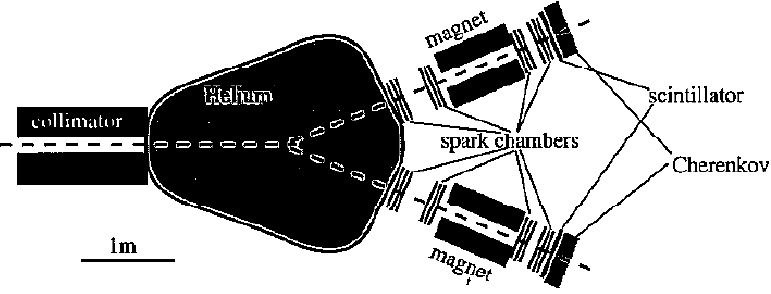
\includegraphics[width=0.7\linewidth]{cp_violation/kaon_verval_exp.png}
    \caption{Onderzoek naar het verval van $K$ mesonen}%
    \label{fig:cp_violation/kaon_verval_exp}
\end{figure}

De binnenkomende $K_L^0$'s vervallen in de helium kamer en worden opgevangen door 2 magneten, één voor $\pi^+$ en één voor $\pi^-$. We verwachten dat dit verval zowel een $\pi^+$, een $\pi^-$ en een $\pi^0$ heeft. Bij het recombineren van de waargenomen $\pi^+$ en $\pi^-$ verwachten we dus niet dat dit volledig overeen zullen komen met de massa van $K_L^0$ (135MeV moet aan $\pi^0$ meegegeven worden). Kijken we nu naar de resultaten in figuur \ref{fig:cp_violation/kaon_verval_exp_res} zien we resultaten die we niet zouden verwachten. Als de massa van de samengestelde pionen buiten de zone van de eigenmassa van $K_L^0$ liggen zijn deze mooi uniform in functie van de hoek waaronder ze van elkaar weg gaan. Dit is niet het geval als hun samengestelde massa gelijk is aan de rustmassa van $K_L^0$. Hier krijgen we een piek voor als ze in elkaars tegengestelde richting vervallen. Dit wil dus zeggen dat $K_L^0$ is vervallen in alleen $\pi^+\pi^-$. Dit toont aan dat de $CP$ wordt geschonden met een branching ratio: $B\left(K_{L}^{0} \rightarrow 2 \pi\right)=2 \times 10^{-3} \neq 0$

\begin{figure}[h]
    \centering
    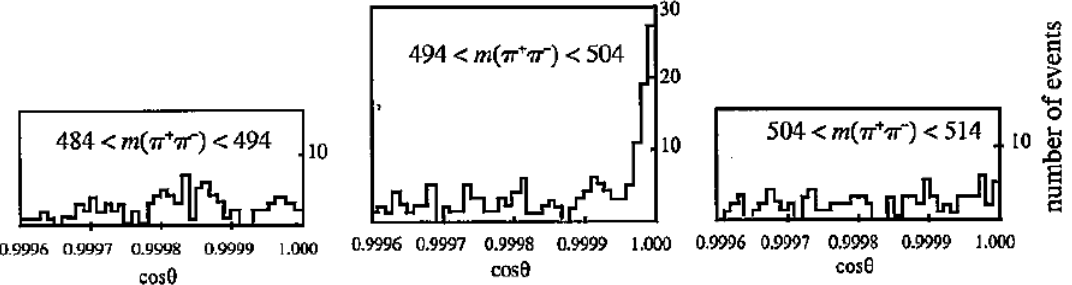
\includegraphics[width=0.8\linewidth]{cp_violation/kaon_verval_exp_res.png}
    \caption{Resulaten van het kaon verval onderzoek}%
    \label{fig:cp_violation/kaon_verval_exp_res}
\end{figure}

\subsection{Mogelijkheden tot $CP$ schending}%
\label{sub:mogelijkheden_tot_cp_schending}

Er zijn verschillende manieren om aan $CP$ schending in het vorige experiment te verklaren.
\begin{itemize}
    \item De $K_S^0$ en $K_L^0$ zijn geen $CP$ eigentoestanden. Dit noemen we de indirecte CP schending.
    \item $CP$ schending in het verval. Het is de interactie verantwoordelijk voor dit verval, de zwakke wisselwerking, schendt $CP$ rechtstreeks. Dit noemen we direct CP verval.
    \item Interferentie met oscillaties. Hier komen we later op terug
\end{itemize}

\subsection{Kaon systeem}%
\label{sub:kaon_systeem}

Onderzoeken we nu deze mogelijke manieren om de $CP$ te schenden op het kaon systeem. Eerst onderzoeken we de indirecte schending. We veronderstellen de de vrije kaonen zijn $CP$ eigentoestanden en dat $K_S^0\neq K_1^0$ en $K_L^0\neq K_2^0$ zijn. Dit voeren we in door de $CP$ eigentoestanden op te mengen. Bij deze opmengingen wordt er telkens maar een kleine fractie $\epsilon$ van de andere eigentoestand toegevoegd.
\begin{equation}
    \begin{aligned}
        \label{eq:kaon_indirecte_cp_violation_1}
        \left| K_{S}^{0}\right>&=\frac{1}{\sqrt{1+|\epsilon|^{2}}}\left(\left|K_{1}^{0}\right>+\epsilon\left| K_{2}^{0} \right>\right) \\
                               &=\frac{1}{\sqrt{2\left(1+|\epsilon|^{2}\right)}}\left(\left|K^{0}\right>+\left| \bar{K}^{0}\right>+\epsilon\left(\left|K^{0}\right>-\left| \bar{K}^{0}\right>\right)\right) \\
                               &=\frac{1+\epsilon}{\sqrt{2\left(1+|\epsilon|^{2}\right)}}\left|K^{0}\right>+\frac{1-\epsilon}{\sqrt{2\left(1+|\epsilon|^{2}\right)}}\left| \bar{K}^{0}\right>\\
                               &=p_{K}\left|K^{0}\right>+q_{K}\left| \bar{K}^{0}\right>\\
        \left| K_{L}^{0}\right>=& \frac{1}{\sqrt{1+|\epsilon|^{2}}}\left(\epsilon\left|K_{1}^{0}\right>+\left| K_{2}^{0}\right>\right) \\
                                &=p_{K}\left|K^{0}\right>-q_{K}\left| \bar{K}^{0}\right>
    \end{aligned}
\end{equation}
Herschrijven we deze schending nu tot $\eta_{+-}$ en dus in functie van de fase dan vinden we:
\begin{equation}
    \begin{aligned}
        \label{eq:kaon_indirecte_cp_violation_2}
        \eta_{+-} &=\left|\eta_{+-}\right| e^{i \delta_{+-}}=\frac{A\left(K_{L}^{0} \rightarrow \pi^{+} \pi^{-}\right)}{A\left(K_{S}^{0} \rightarrow \pi^{+} \pi^{-}\right)} \\
        \left|\eta_{+-}\right|^{2} &=\frac{\Gamma\left(K_{L}^{0} \rightarrow \pi^{+} \pi^{-}\right)}{\Gamma\left(K_{S}^{0} \rightarrow \pi^{+} \pi^{-}\right)} \\
        \eta_{00} &=\left|\eta_{00}\right| e^{i \delta_{00}}=\frac{A\left(K_{L}^{0} \rightarrow \pi^{0} \pi^{0}\right)}{A\left(K_{S}^{0} \rightarrow \pi^{0} \pi^{0}\right)} \\
        \left|\eta_{00}\right|^{2} &=\frac{\Gamma\left(K_{L}^{0} \rightarrow \pi^{0} \pi^{0}\right)}{\Gamma\left(K_{S}^{0} \rightarrow \pi^{0} \pi^{0}\right)}
    \end{aligned}
\end{equation}
De $A$ refereert hier naar amplitudes die in een ratio herleid kunnen worden tot hun verval breedtes. Voor $\eta_{+-}$ is het verval in  de teller verboden volgens $CP$ en de noemer toegelaten. De $\eta_{00}$ doet hetzelfde maar dan voor het verval naar $\pi^0\pi^0$. Indien $\eta_{+-}=\eta_{00}=\epsilon$ dan hebben we enkel indirecte $CP$ schending. Indien deze niet $\eta$'s niet gelijk zijn aan elkaar zal er ook directe $CP$ schending voorkomen.\\
{\color{red} Er wordt hier voor deze vergelijkingen niet verwacht dat je ze volledig kan uitwerken en opschrijven. Er wordt wel verwacht dat je het verhaal kan vertellen dat $\eta_{+-}$ overeen komt met de $\pi^+\pi^-$ vervallen en $\eta_{00}$ voor het verval naar $\pi^0\pi^0$. En dat het verschil tussen de 2 uiteindelijk overeen komt met de direct vs indirecte CP schending. Je moet ook kunnen zeggen wat deze 2 soorten CP schending zijn.}\\
In het meest algemene geval krijgen we:
\begin{equation}
    \begin{aligned}
        \label{eq:direct_indirect_algemeen}
        \eta_{+-} &=\epsilon+\epsilon^{\prime} \\
        \eta_{00} &=\epsilon-2 \epsilon^{\prime}
    \end{aligned}
\end{equation}
met $\epsilon$ de indirecte $CP$ schending en $\epsilon'$ de directe. Om het verschil tussen $\epsilon$ en $\epsilon'$ te weten moeten we de $\eta$'s meten.

\subsubsection{Experiment}%
\label{ssub:experiment}

We moeten dus onderzoek doen naar $K^{0} \rightarrow \pi \pi$ met de pion zowel geladen als neutraal. Die zijn vroeger al gedaan maar worden tot de dag van vandaag nog steeds verbetert. We hebben vandaag de dag voor de $\eta$'s de volgende resultaten:
\begin{equation}
    \begin{aligned}
        \label{eq:hedendaagse_eta}
        \left|\eta_{+-}\right| &=(2.232 \pm 0.011) \times 10^{-3} \\
        \left|\eta_{00}\right| &=(2.220 \pm 0.011) \times 10^{-3}
    \end{aligned}
\end{equation}
Om tot deze waarschijnlijkheid te meten is heel veel experimentele ingeniositeit aan te pas moeten komen. Desondanks de vele uren en energie dat hier in gestoken zijn is het niet goed genoeg om te zien of er indirecte $CP$ schending is. We zijn met deze metingen 100\% zeker dat er $CP$ schending is maar om te zien of we aan directe $CP$ schending doen, moet er met nog hogere precisie gemeten worden. Wat we nu zo precises willen meten is de ratio tussen de $\eta$'s.
\begin{equation}
    \begin{aligned}
        \label{eq:eta_ratio}
        R&=\left|\frac{\eta_{00}}{\eta_{+-}}\right|^{2}\\
         &=\frac{\Gamma\left(K_{L} \rightarrow \pi^{0} \pi^{0}\right)}{\Gamma\left(K_{L} \rightarrow \pi^{+} \pi^{-}\right)} \cdot \frac{\Gamma\left(K_{S} \rightarrow \pi^{+} \pi^{-}\right)}{\Gamma\left(K_{S} \rightarrow \pi^{0} \pi^{0}\right)} \\
         &=\left|\frac{\epsilon-2 \epsilon^{\prime}}{\epsilon+\epsilon^{\prime}}\right|^{2}=\left|\frac{1-2 \epsilon^{\prime} / \epsilon}{1+\epsilon^{\prime} / \epsilon}\right|^{2} \\
         &\approx\left|1-3 \frac{\epsilon^{\prime}}{\epsilon}\right|^{2} \approx 1-3\left(\frac{\epsilon^{\prime}}{\epsilon}+\frac{\epsilon^{\prime *}}{\epsilon^{*}}\right) \\
         &=1-6 \Re\left(\frac{\epsilon^{\prime}}{\epsilon}\right)
    \end{aligned}
\end{equation}
De reden waarom we overstappen naar deze ratio is omdat $\frac{\Gamma\left(K_{L} \rightarrow \pi^{0} \pi^{0}\right)}{\Gamma\left(K_{L} \rightarrow \pi^{+} \pi^{-}\right)}$ en $\frac{\Gamma\left(K_{S} \rightarrow \pi^{+} \pi^{-}\right)}{\Gamma\left(K_{S} \rightarrow \pi^{0} \pi^{0}\right)}$ veel preciser kunnen bepaalt worden dan $\eta_{+-}$ en $\eta_{00}$.\\
Dit is een heel typisch voorbeeld van dubbele ratios die gebruikt worden om veel nauwkeurigere metingen te doen omdat we de tellers en noemers kunnen herschikken in ons voordeel. In dit geval zullen door de herschikte ratios de fluxen van $K_L^0$ en $K_S^0$ wegvallen.\\
Zo was het uiteindelijk mogelijk om deze ratio heel exact te gaan meten.
\begin{equation}
    \begin{aligned}
        \label{eq:eta_ratio_results}
        \left|\frac{\eta_{00}}{\eta_{+-}}\right| &=0.9951 \pm 0.0008(\neq 1) \\
        \Re\left(\frac{\epsilon^{\prime}}{\epsilon}\right) &=(1.65 \pm 0.26) \times 10^{-3} \\
        |\epsilon| &=(2.228 \pm 0.011) \times 10^{-3}
    \end{aligned}
\end{equation}
Het is vandaag de dag dus duidelijk dat er zowel direct als indirecte $CP$ schending zal plaats vinden.

\end{document}
